%% Begin copyright
%%
%%  /home/jrf/Documents/books/Books20/Docs/Hjs/hjs_catalogue.tex
%%
%%   Part of the Books20 Project
%%
%%   Copyright 2022 James R. Fowler
%%
%%   All rights reserved. No part of this publication may be
%%   reproduced, stored in a retrival system, or transmitted
%%   in any form or by any means, electronic, mechanical,
%%   photocopying, recording, or otherwise, without prior written
%%   permission of the author.
%%
%%
%% End copyright
%
% History
% created 11 June 2022
%
%----------------------------------------------------------
\documentclass[letterpaper]{book}

\usepackage[paper=letterpaper,twoside]{geometry}
\usepackage[T1]{fontenc}

\usepackage{graphicx}
\usepackage{wrapfig}
\usepackage[noautomatic]{imakeidx}
%\usepackage{imakeidx}
\usepackage[titlesize=12pt,parsize=10pt]{colophon}
\usepackage{books20}
\addglobalbib{../MasterBib.bib}
\addbibresource{hjs_baas_obit.bib}
\addbibresource{hjs.bib}

\newcommand*{\myhref}[1]{\hyperlink{entry:#1}{#1}}

\makeindex[name=author,title=Author/Editor Index]

\begin{document}

\frontmatter
% Half-Title page
\thispagestyle{empty}
\vspace*{1 in}
\begin{centering}
  \textsc{\Large Catalogue of the Harlan J.~Smith Collection}
\end{centering}
\newpage

% Title page
\thispagestyle{empty}
\title{\textsc{Catalogue of the \\
    Harlan J.\ Smith Collection \\
    of Science Books \\
    in the Otto Struve Library of \\
    the McDonald Observatory \\
    Fort Davis, Texas}}
\author{compiled by James R. Fowler}
\date{copy of \today}
\maketitle
\newpage
% copyright page
\thispagestyle{empty}
\vspace*{5 in}
\centerline{Copyright \copyright\ 2023 McDonald Observatory}
\centerline{Fort Davis, Texas}
\newpage

% Dedication and acknowledgement
%%\vspace*{3 in}
\newgeometry{inner=2in, outer=2in,top=4in}
\thispagestyle{empty}
\noindent
The McDonald Observatory would like to thank Joan Smith,
Nat Smith, and the rest of the Harlan J.~Smith family
for generously donating this collection to the observatory.
This collection will be of scientific as well as historic
interest to the staff and visitors of the observatory.
\restoregeometry
\newpage

\thispagestyle{empty}
\begin{figure}[t]
  \centering
  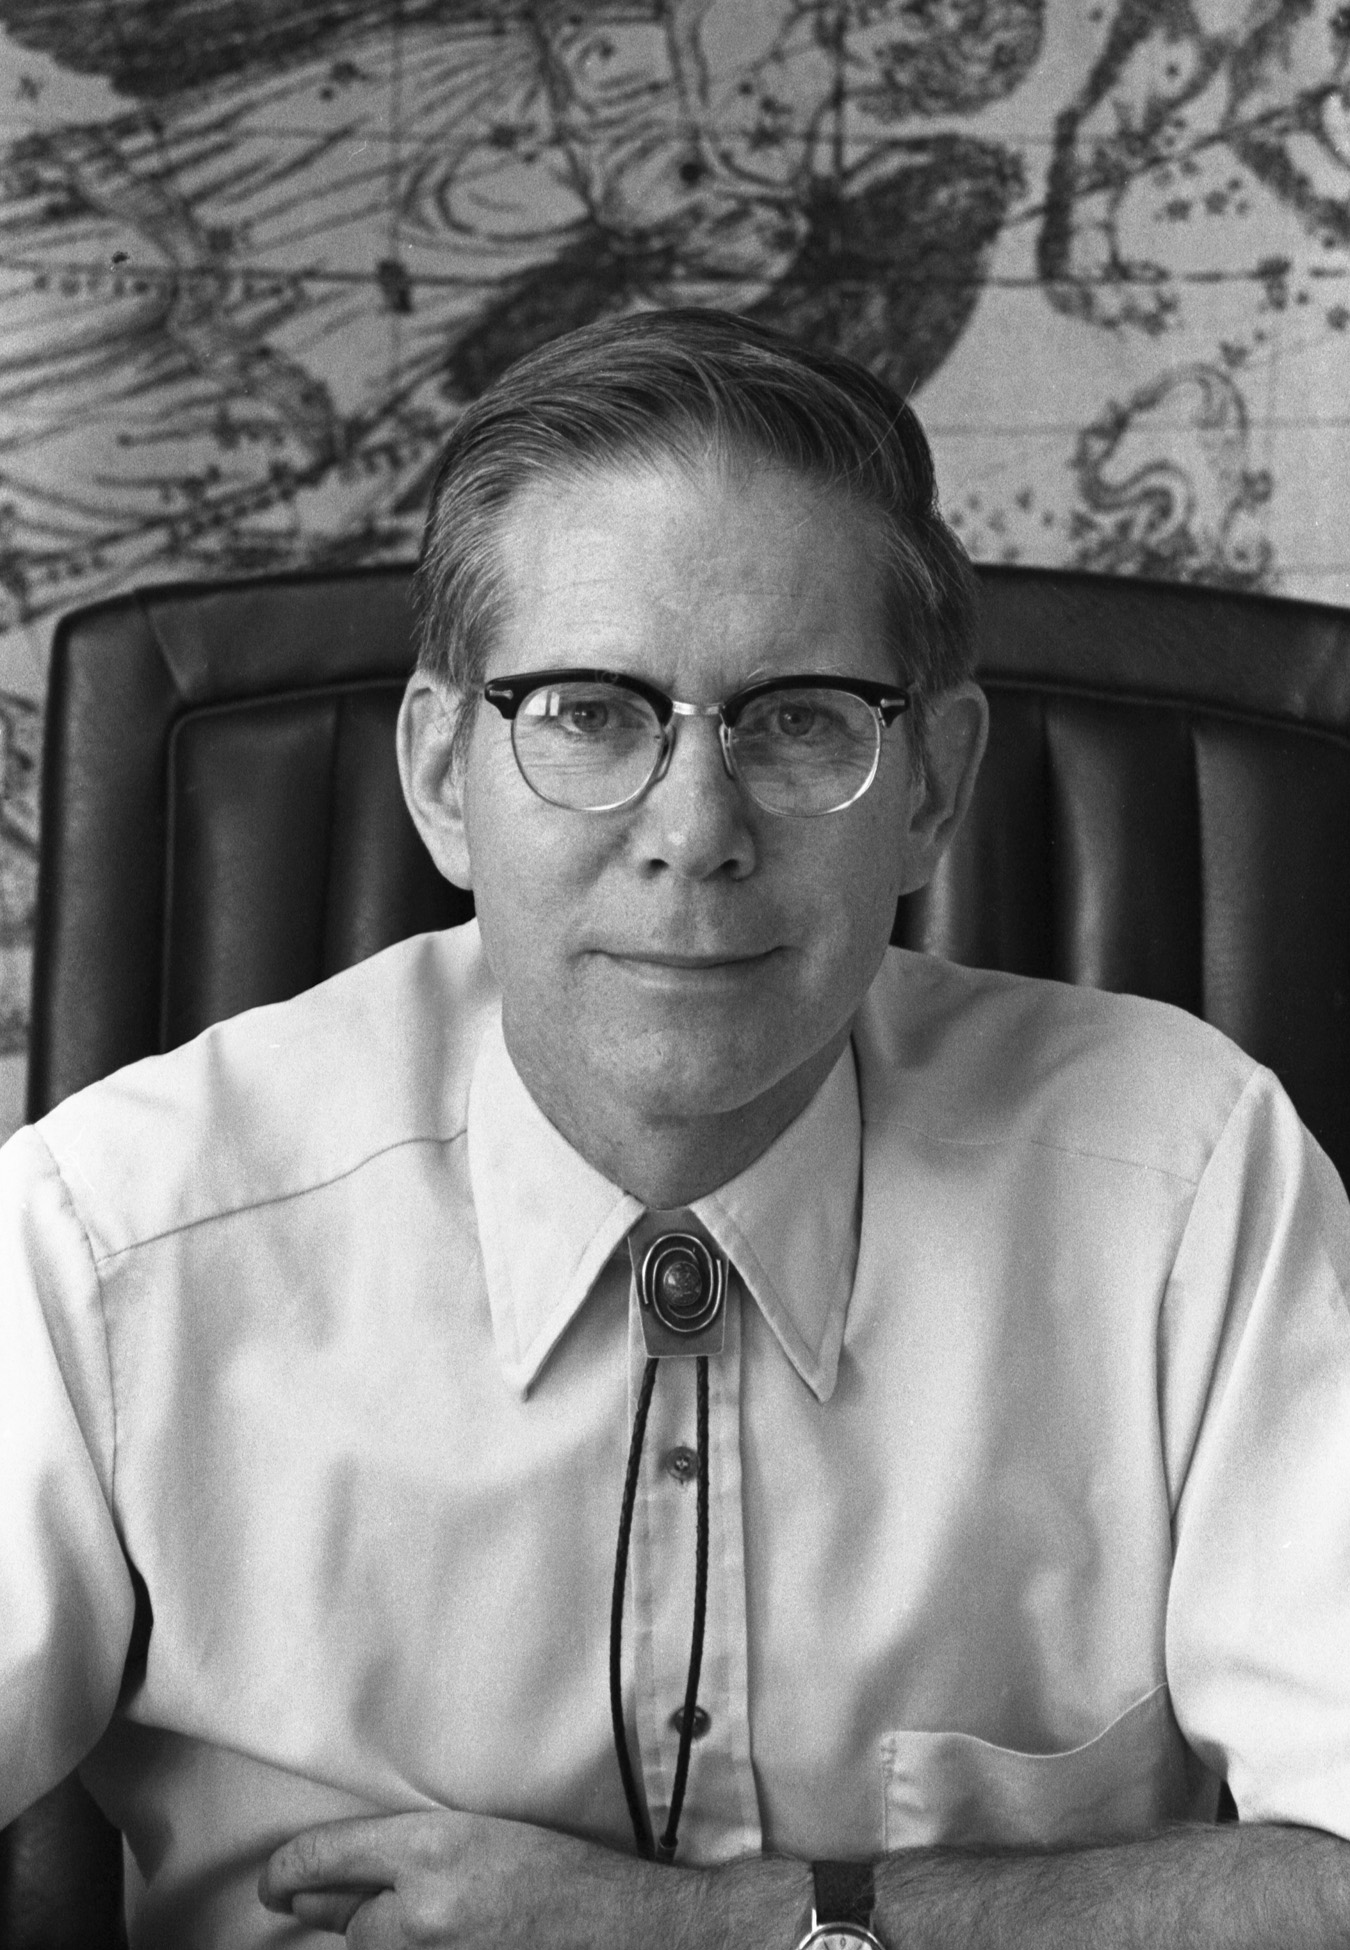
\includegraphics{hjs_photo.jpg} \\
  Harlan J.~Smith 1924 -- 1991 \\
  {\scriptsize from Wikipedia
    (https://en.wikipedia.org/wiki/Harlan\_James\_Smith \\
    \href{https://creativecommons.org/licenses/by-sa/4.0}{License CC by-sa 4.0}}
  \label{fig:hjs}
\end{figure}
\clearpage
%\mbox{}
%\thispagestyle{empty}
%\newpage

\pagestyle{plain}
\vspace*{1 in}
\centerline{\Large \bf Harlan J.\ Smith}
\bigskip\bigskip
\import{./}{biography}
\newpage

\vspace*{1 in}
\centerline{\Large \bf The Books}
\bigskip\bigskip
\import{./}{library}
\newpage
%%\showthe\font

\printbibliography

\mainmatter
\begin{center}
  {\Large \bf Catalogue of the Harlan J.\ Smith Collection}
\end{center}
\bigskip
\import{./}{books}

%%\showthe\font

\backmatter

\indexprologue{This index gives the catalogue entry numbers where the
  particular author/editor(s) can be found.}  \printindex[author]

\begin{colophon}
  The catalogue was typeset with the \LaTeX2e\ processing system in
  10pt Computer Modern Roman font. It has been printed and
  bound by J.~Fowler.
\end{colophon}

\end{document}

